% ----------------------------------------------------------
% Apêndices
% ----------------------------------------------------------

% ---
% Inicia os apêndices
% ---
\begin{apendicesenv}

% Imprime uma página indicando o início dos apêndices
\partapendices

% ----------------------------------------------------------
\chapter{Diagrama da estrutura do currículos Lattes}
\label{ap:diagramacurriculo}
% ----------------------------------------------------------

\begin{figure}[htpb]
  \centering
  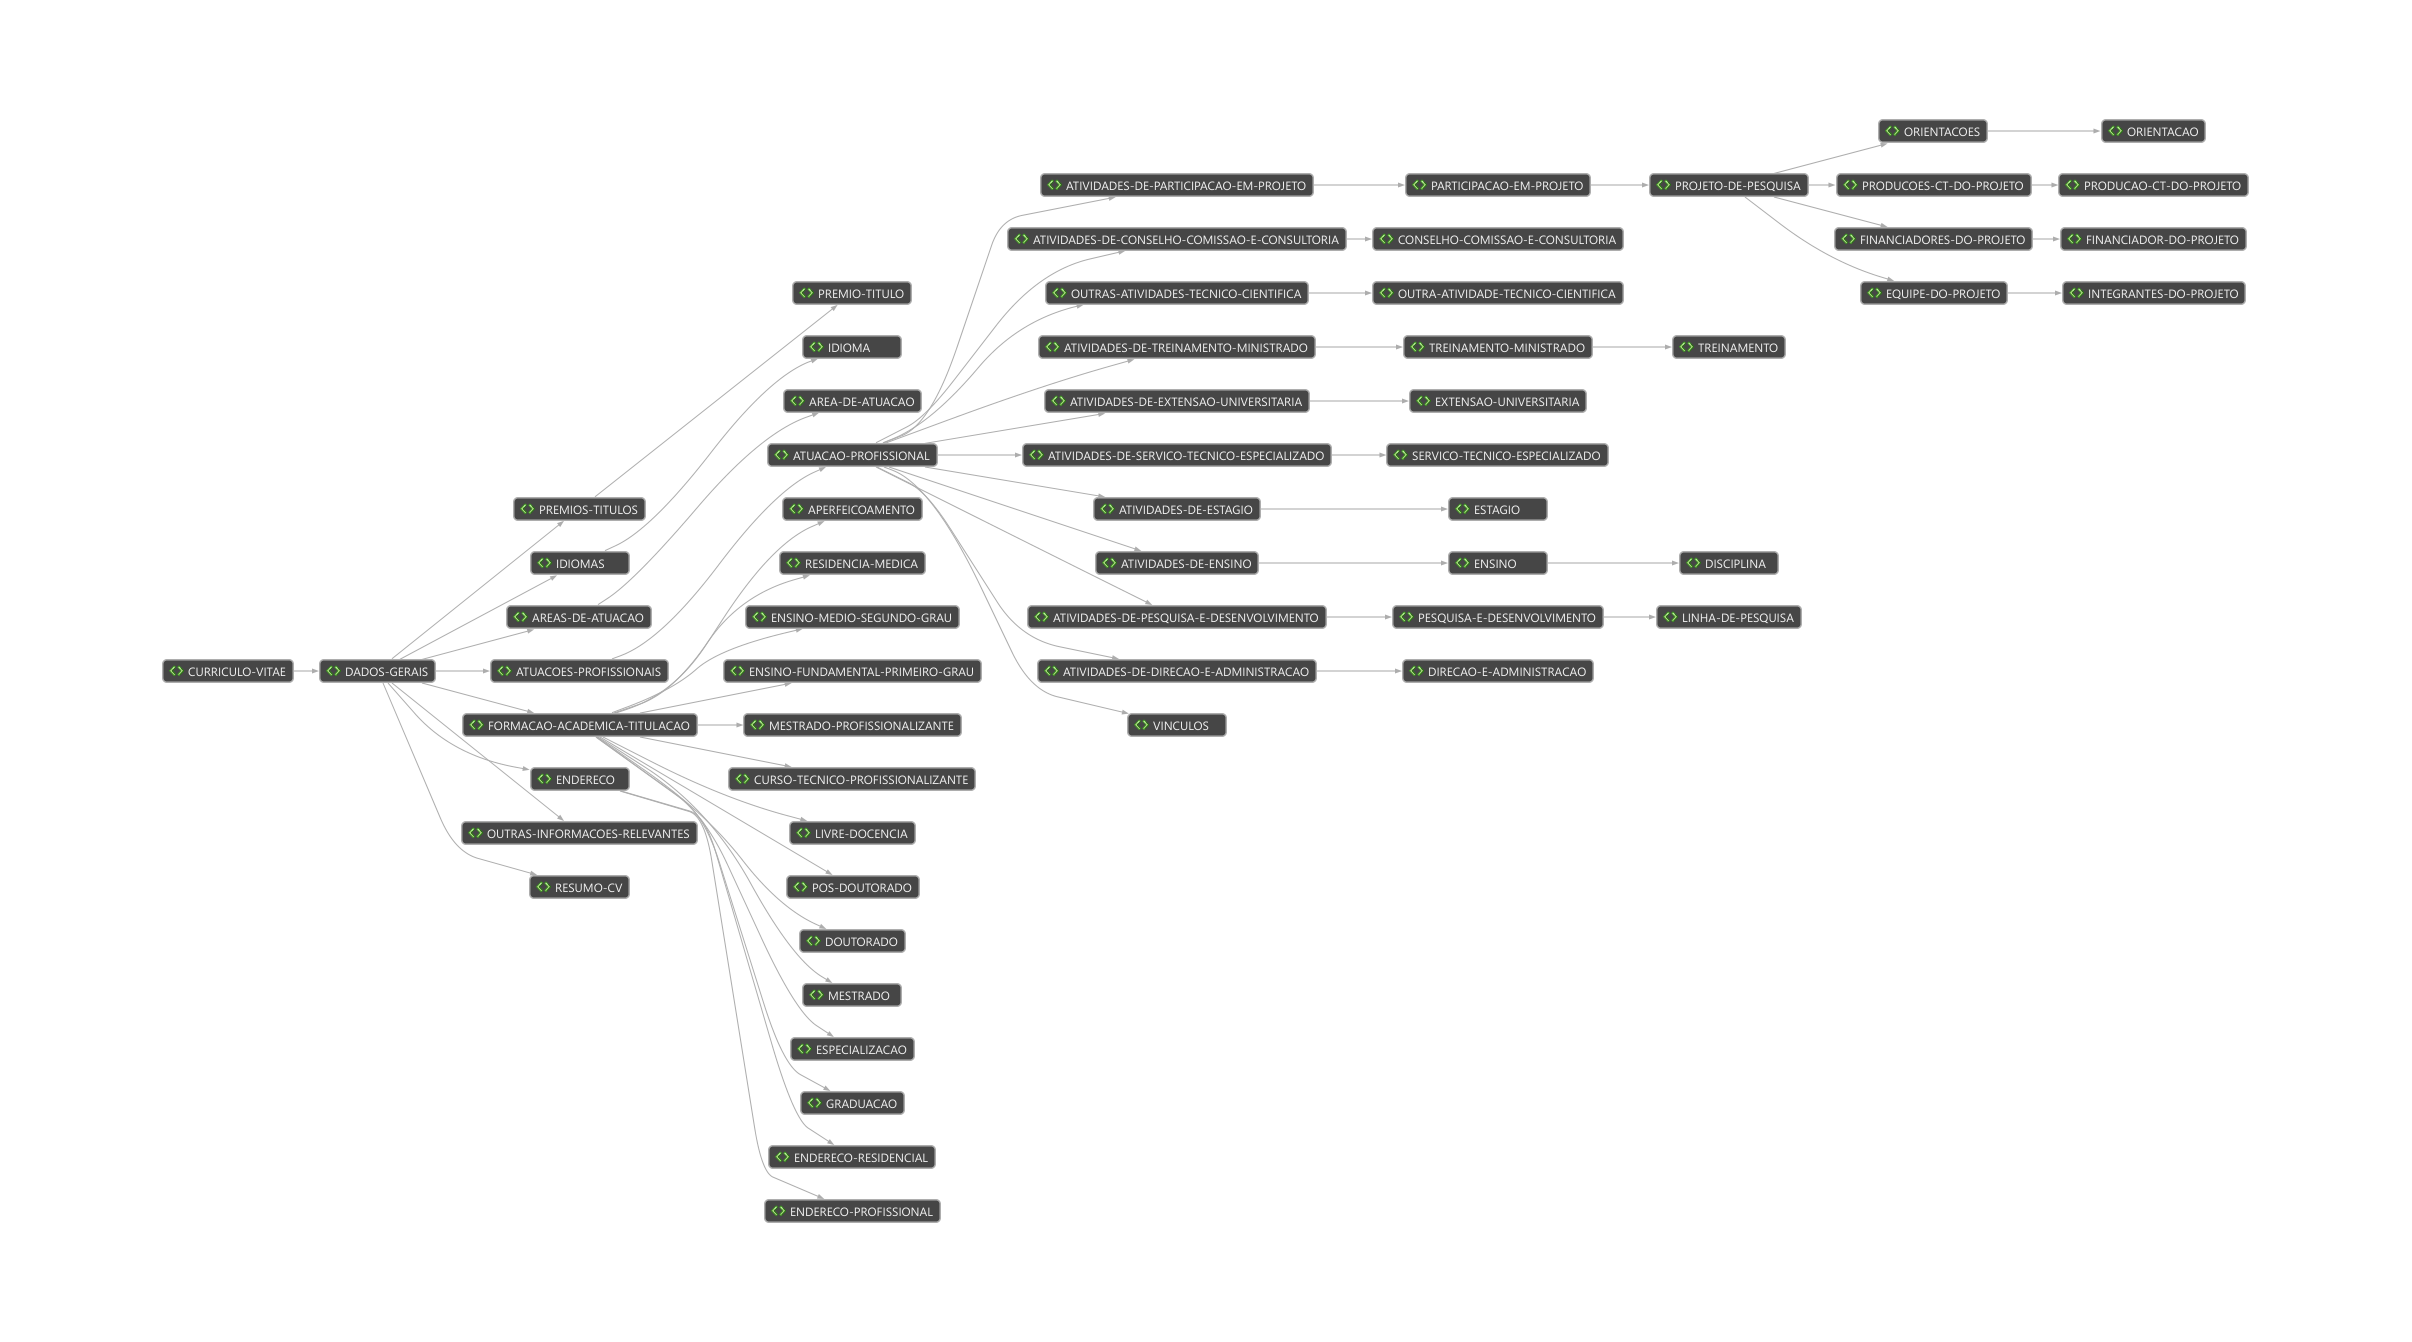
\includegraphics[width=1\textwidth]{figuras/diagrama-curriculo-dados-gerais}
  \caption{Uma visão geral dos nós do currículo Lattes relativos aos dados do pesquisador.}
  \label{fig:diagramadadosgerais}
\end{figure}

\begin{figure}[htpb]
  \centering
  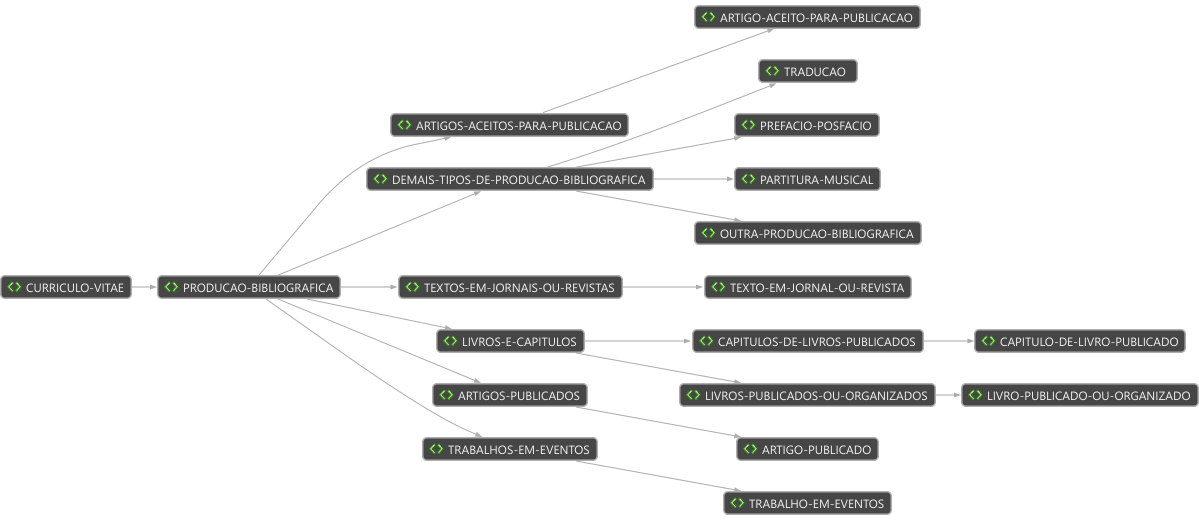
\includegraphics[width=1\textwidth]{figuras/diagrama-curriculo-producao-bibliografica}
  \caption{Uma visão geral dos nós do currículo Lattes relativos à produção bibliográfica.}
  \label{fig:diagramaproducaobibliografica}
\end{figure}

% ----------------------------------------------------------
\chapter{Diagrama entidade-relacionamento do banco de dados completo}
% ----------------------------------------------------------

% ----------------------------------------------------------
\chapter{Exemplos de coautorias identificadas na etapa de transformação do método}
% ----------------------------------------------------------

% ----------------------------------------------------------
\chapter{Exemplos de áreas de atuação do pesquisador inferidas na etapa de transformação do método}
% ----------------------------------------------------------

\end{apendicesenv}
% ---